\documentclass[11pt,a4paper]{article}

\usepackage[utf8]{inputenc}
\usepackage[T1]{fontenc}
\usepackage[spanish,es-nodecimaldot,es-noshorthands]{babel}
\usepackage{lmodern}
\usepackage[margin=2.3cm]{geometry}
\usepackage{amsmath,amssymb}
\usepackage{graphicx}
\usepackage{booktabs}
\usepackage{tabularx}
\usepackage{array}
\usepackage{float}
\usepackage{caption}
\usepackage{enumitem}
\usepackage[hidelinks]{hyperref}

\graphicspath{{figuras/}}
\captionsetup{font=small,labelfont=bf}
\setlist{itemsep=2pt,topsep=4pt}

\newcommand{\uA}{\,\mu\mathrm{A}}
\newcommand{\GHz}{\,\mathrm{GHz}}
\newcommand{\MHz}{\,\mathrm{MHz}}
\newcommand{\kHz}{\,\mathrm{kHz}}
\newcommand{\mK}{\,\mathrm{mK}}
\newcommand{\dBm}{\,\mathrm{dBm}}
\newcommand{\dB}{\,\mathrm{dB}}
\newcommand{\fr}{f_r}
\newcommand{\dfr}{\delta\!f_r}

\title{Chip fluxonium: mediciones de los resonadores de lectura,\\
espectroscopía de uno y dos tonos con flujo, y por qué no se pudo\\
confirmar un qubit funcionando}
\author{Mediciones de octubre y noviembre de 2026}
\date{13 de noviembre de 2026}

\begin{document}
\maketitle

\begin{abstract}
\noindent
Se caracterizaron los resonadores de lectura de un chip con qubits tipo fluxonium y se buscó la señal de los
qubits por espectroscopía de un tono (corrimiento del resonador con el flujo) y de dos tonos (drive por una antena
y lectura dispersiva), con una bobina externa para variar el flujo. Los resonadores responden al flujo con ramas
parabólicas periódicas e histeréticas (período $\approx 50\uA$), propias de un lazo superconductor con estados de
fluxoide metaestables, y en el resonador de Q4 aparece además una oscilación suave de $23.8\uA$ de período. Sin
embargo, ninguna medición mostró una transición espectral que dependa del flujo. En la medición más sensible
(ruido de $\sim 2\kHz$ por punto en el corrimiento de $\fr$, drive de $1\MHz$ a $4\GHz$, más de un período de flujo
esperado) no hay nada que cambie con la corriente de la bobina por encima de $\sim 3$--$4\kHz$. Solo aparecen tres
líneas fijas (0.293, 2.81 y $3.276\GHz$) con la firma de absorción o calentamiento. Con estos datos no se puede
confirmar que haya un qubit funcionando; se discuten las hipótesis físicas que explican lo medido y lo que haría
falta para resolverlo.
\end{abstract}

\tableofcontents
\newpage

%==============================================================================
\section{Objetivo y contexto}
%==============================================================================

El chip contiene qubits fluxonium (Q1--Q4), cada uno acoplado a un resonador de lectura de guía de onda coplanar.
Un fluxonium es un lazo superconductor formado por una juntura chica en paralelo con una superinductancia (un arreglo
de junturas). Sus parámetros de diseño son del orden de $E_J \approx 8\GHz$ y $E_L \approx 0.8\GHz$
($E_J/E_L \approx 10$). El espectro depende del flujo externo $\Phi_{\rm ext}$ a través del lazo con período de un
cuanto $\Phi_0 = h/2e$, y la transición $0\to1$ es mínima en medio cuanto ($\Phi_0/2$), donde típicamente vale unos
cientos de MHz.

El objetivo fue encontrar esa transición. Para eso:
\begin{enumerate}
  \item se caracterizaron los resonadores de lectura (frecuencia, factores de calidad, número de fotones);
  \item se midió la respuesta de los resonadores al flujo aplicado con una bobina externa;
  \item se buscó la modulación periódica de $\fr$ con el flujo (espectroscopía de un tono);
  \item se buscó la transición del qubit con un segundo tono por la antena de drive (espectroscopía de dos tonos).
\end{enumerate}

Según la información de fabricación, el chip no salió como se esperaba: los resonadores quedaron con factores de
calidad bajos (líneas anchas, $\kappa/2\pi$ de 6 a $16\MHz$) y los qubits, en principio, muy desacoplados de sus
resonadores. Eso hace que cualquier señal esperable sea muy chica.

%==============================================================================
\section{Montaje experimental}
%==============================================================================

\begin{itemize}
  \item \textbf{Criostato:} refrigerador de dilución Bluefors. La placa de mezcla (MXC) está a $\approx 8.0\mK$ sin
    medir y a $8.5$--$10\mK$ durante las mediciones con drive (sección~\ref{sec:temperatura}).
  \item \textbf{Lectura:} VNA Keysight PNA N5245A. Atenuación de entrada total de $-112\dB$ (62\,dB externos y
    50\,dB en la línea del criostato); algunas mediciones usaron $-81\dB$ o $-50\dB$. La salida tiene un HEMT y,
    antes del amplificador de temperatura ambiente, un filtro pasabanda de 5.7--7\,GHz.
  \item \textbf{Drive:} generador Keysight N5173B por la antena del qubit, con 20\,dB de atenuación hasta la antena.
  \item \textbf{Flujo:} bobina externa alimentada por una fuente de corriente Keithley, con rampas siempre lentas y
    acercándose a cada corriente desde el mismo lado cuando hizo falta (hay histéresis).
  \item \textbf{Software:} módulos de Python sobre QCoDeS (\texttt{vna\_single.py}, \texttt{barrido\_flujo.py},
    \texttt{fit\_resonancia.py}, \texttt{dos\_tonos.py}); todo queda en bases SQLite con la metadata de cada run.
\end{itemize}

\paragraph{Número de fotones.} Con el modelo de resonador notch, $\langle n\rangle = 2P_{\rm in}Q_l^2/(Q_c\hbar\omega_0^2)$.
Para el resonador de Q4 con $-112\dB$ de entrada: $\langle n\rangle \approx 0.02$ a $-30\dBm$, $1.7$ a $-10\dBm$,
$17$ a $0\dBm$ y $170$ a $+10\dBm$ en el VNA.

\paragraph{Conversión de $S_{21}$ a corrimiento de $\fr$.} En las mediciones en CW se lee $S_{21}$ a una frecuencia fija
$f_{\rm CW}$ cerca de la resonancia. Con el ajuste notch de una traza de búsqueda se calcula $dS_{21}/df$ en
$f_{\rm CW}$ y cada cambio $\Delta S_{21}$ se proyecta como
\begin{equation}
  u = \frac{\Delta S_{21}}{dS_{21}/df}, \qquad \dfr = -\mathrm{Re}\,u, \qquad \text{pérdida} = \mathrm{Im}\,u,
\end{equation}
es decir, en un corrimiento equivalente de la frecuencia del resonador (dispersivo) y en una componente ortogonal
(cambio de pérdidas). Ambas se expresan en kHz.

%==============================================================================
\section{Caracterización de los resonadores}
%==============================================================================

En octubre los resonadores eran $\lambda/4$. En noviembre se cortó el corto a tierra y pasaron a $\lambda/2$, con
frecuencias más altas. Los parámetros típicos (ajuste notch de Probst, con asimetría y retardo de cable) son:

\begin{table}[H]
\centering
\begin{tabular}{lcccc}
\toprule
Resonador & $\fr$ [GHz] & $\kappa/2\pi$ [MHz] & $Q_i$ & $Q_c$ \\
\midrule
res\_q1 & 5.4135 & $\approx 10.6$ & $\approx 965$ & -- \\
res\_q2 & 6.0746 & 15.5--15.9 & 665--715 & $\approx 840$ \\
res\_q4 & 5.9922 & 6.1--8 & 1020--1250 & $\approx 2840$ \\
\bottomrule
\end{tabular}
\caption{Resonadores $\lambda/2$ (noviembre). Los $Q$ son bajos para resonadores superconductores; los anchos son
del orden de varios MHz.}
\end{table}

Los barridos en potencia no muestran punch-out ni corrimiento Kerr apreciable: con $-81\dB$ de entrada
($\langle n\rangle \approx 2\times10^3$) y con $-50\dB$ ($\langle n\rangle \approx 2.5\times10^6$) la respuesta del
resonador al flujo es la misma que con $\langle n\rangle \approx 1.7$.

%==============================================================================
\section{Respuesta de los resonadores al flujo}
%==============================================================================

\subsection{Ramas de fluxoide con histéresis}

Al barrer la corriente de la bobina, $\fr$ muestra un diente de sierra: tramos parabólicos separados por saltos
abruptos que se repiten periódicamente, y la posición de los saltos depende del sentido del barrido (histéresis;
figura~\ref{fig:ramas}).

\begin{itemize}
  \item \textbf{res\_q4 ($\lambda/2$):} saltos de $209\pm25\kHz$ con período $T \approx 50$--$52\uA$; histéresis de
    $\approx 0.47$ períodos entre ida y vuelta. Todas las ramas son la misma parábola desplazada,
    $\fr = f_{\rm fondo} - \alpha\,(I-C_n)^2$ con $C_n = x_0 + nT$, que explica el $99.6\,\%$ de la varianza de $\fr$.
    Cada rama existe mientras $|I - C_n| \lesssim 67\uA$ ($\approx 1.3\,T$), de modo que a cada corriente coexisten
    2 o 3 estados.
  \item \textbf{res\_q2:} el mismo período, con saltos más grandes (500--640\,kHz) y curvatura mayor
    ($-136$ contra $-55\,\mathrm{Hz}/\mu\mathrm{A}^2$ en res\_q4).
  \item \textbf{res\_q1:} sin saltos en una ventana de $100\uA$.
  \item \textbf{En $\lambda/4$ (octubre):} saltos de 0.7--1\,MHz con período de 60--65\,$\mu$A.
  \item El patrón no cambia con la potencia de lectura (de $\langle n\rangle \approx 1.7$ a $2.5\times10^6$), y las
    posiciones de los saltos se repiten en corriente absoluta durante horas (entre días se corrieron unos $7\uA$).
\end{itemize}

\begin{figure}[H]
\centering
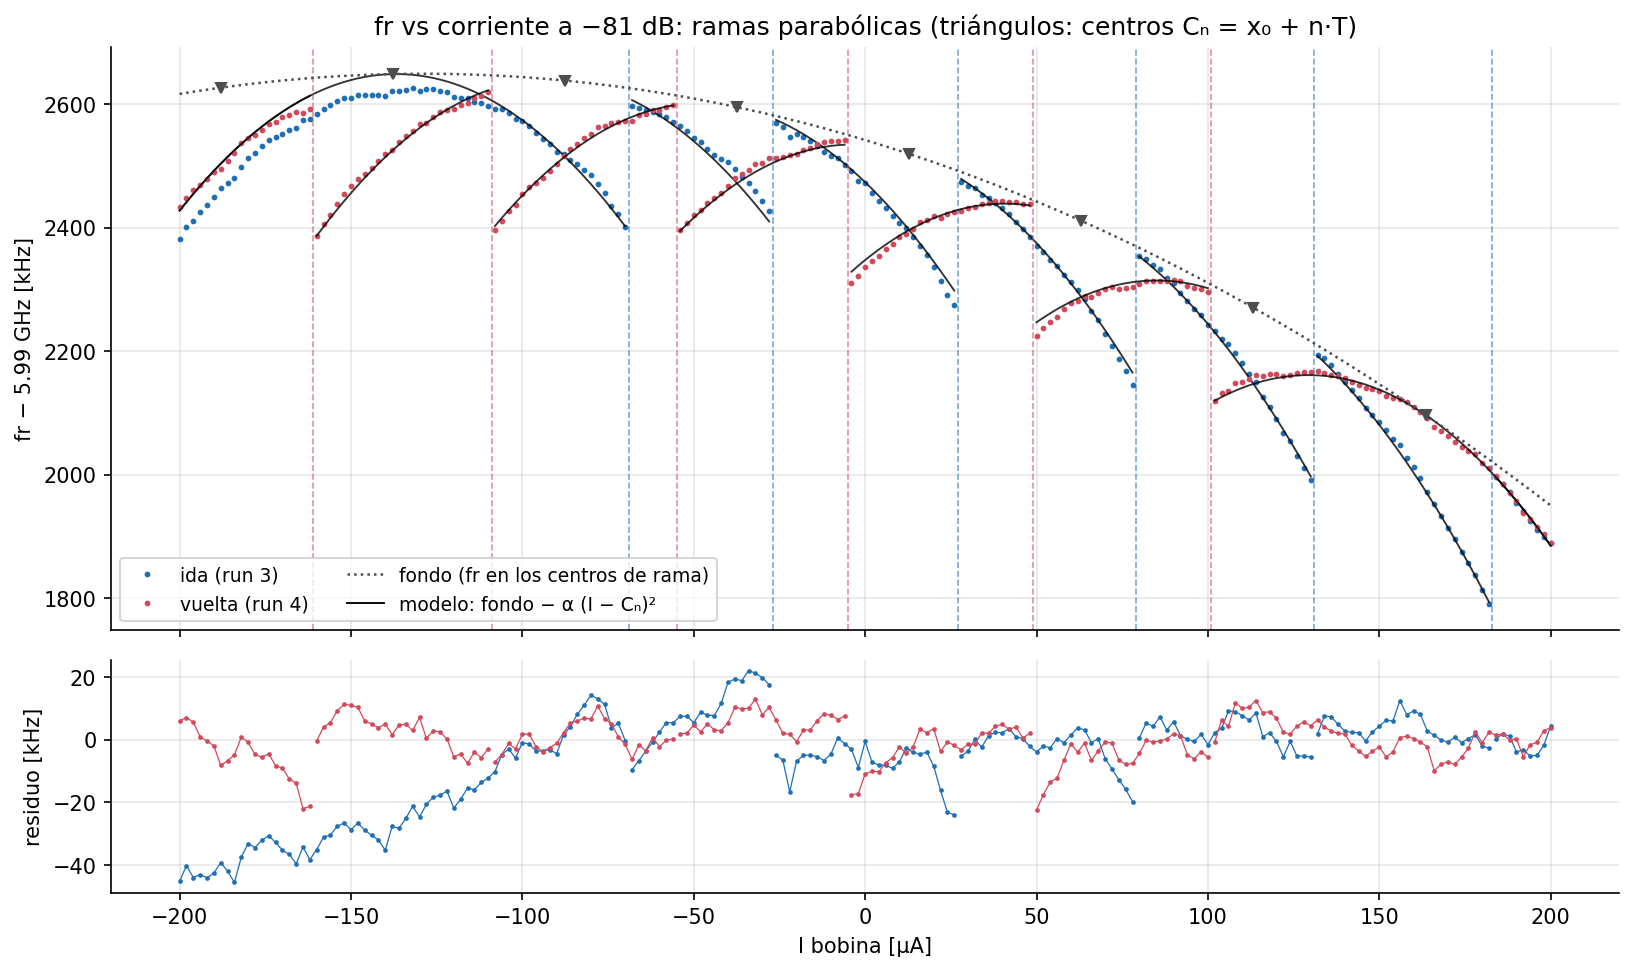
\includegraphics[width=0.92\textwidth]{ramas_fluxoide.png}
\caption{$\fr$ de res\_q4 en función de la corriente de la bobina, ida (azul) y vuelta (rojo), con $-81\dB$ de
entrada. Las curvas negras son el modelo de ramas parabólicas desplazadas un período $T$ entre sí.}
\label{fig:ramas}
\end{figure}

\subsection{Oscilación de $23.8\uA$ en res\_q4}

Después de restar las ramas, los parámetros de res\_q4 oscilan suavemente, sin histéresis, con período
$P = 23.8\uA$ (figura~\ref{fig:osc}): $\pm3.3\kHz$ en $\fr$ ($16\sigma$), $\pm1.6$ en $Q_i$ ($25\sigma$) y
$\approx\pm11\kHz$ en $\kappa/2\pi$, igual en ida y en vuelta.

\begin{itemize}
  \item No aparece en res\_q2 (cota de $0.015\,\%$ en $Q_i$), que según el diseño tiene el mismo qubit. En res\_q1
    queda por debajo de $3\kHz$ en $\fr$.
  \item Desaparece al subir mucho la potencia: con $\langle n\rangle \approx 2.5\times10^6$ su amplitud en $Q_i$ baja
    al menos 9 veces, mientras que las ramas de fluxoide no cambian.
  \item No es un alias de un período más corto: barridos con pasos de 0.25 y $0.5\uA$ no muestran nada entre
    0.55 y $12\uA$.
\end{itemize}

\begin{figure}[H]
\centering
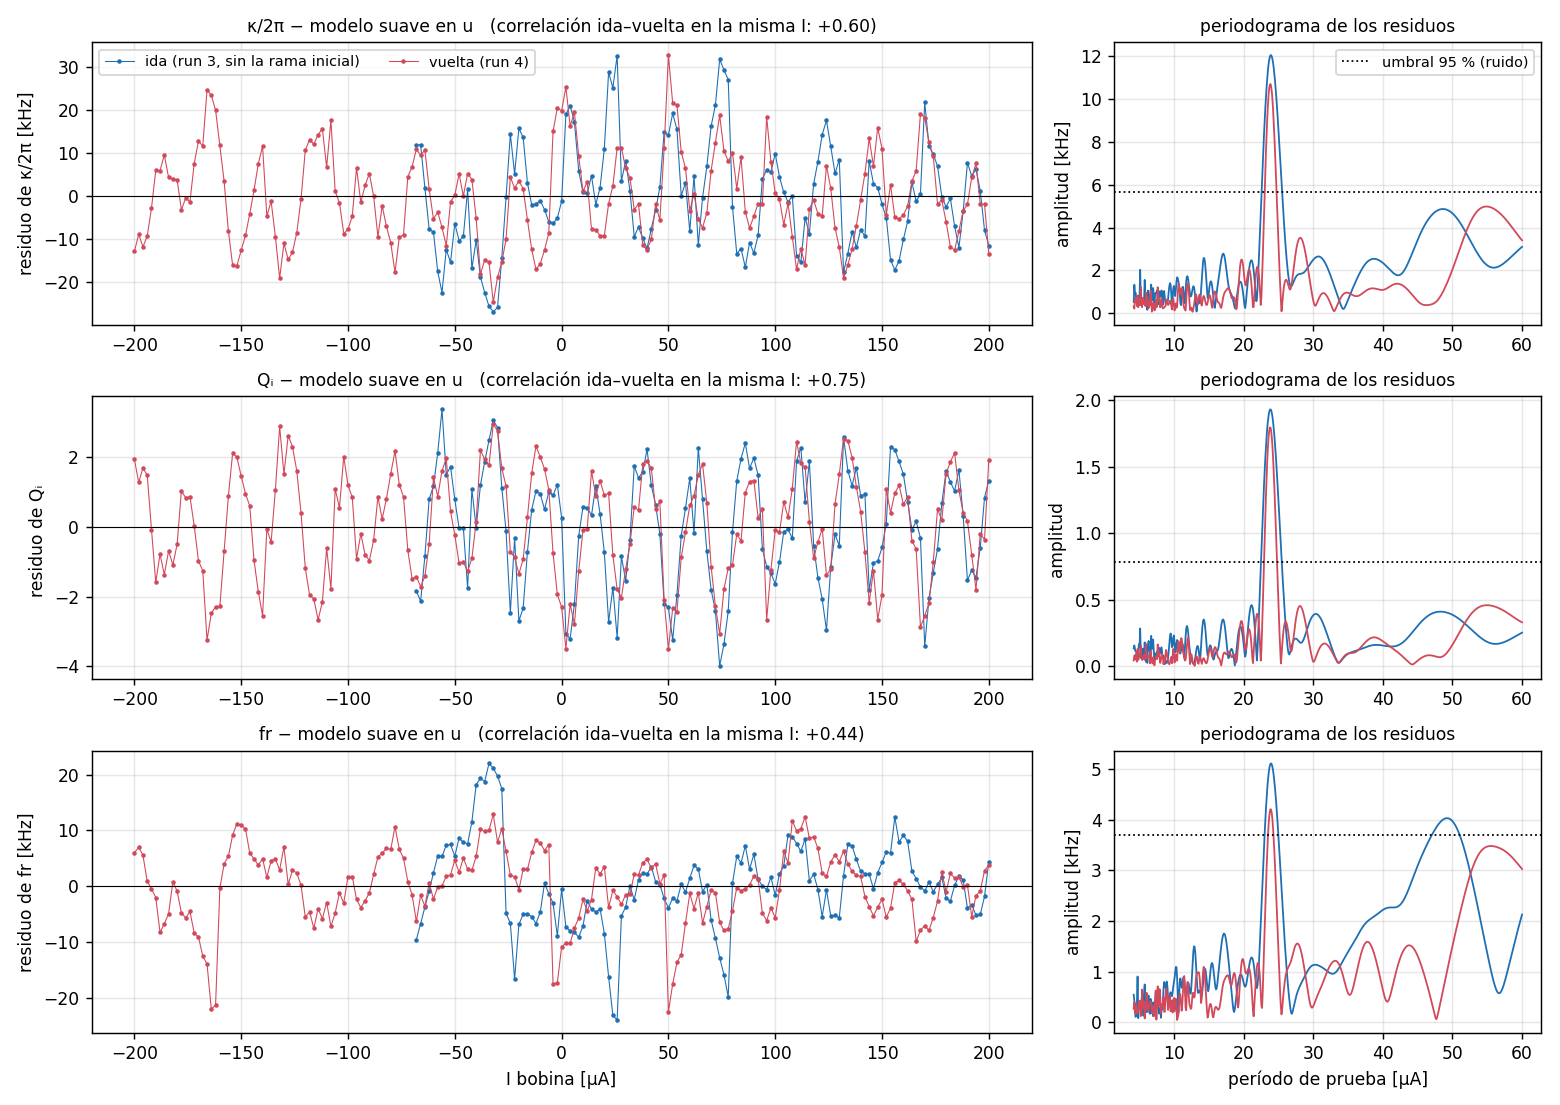
\includegraphics[width=0.95\textwidth]{oscilacion_23uA.png}
\caption{Residuos de $\kappa/2\pi$, $Q_i$ y $\fr$ de res\_q4 después de restar las ramas, y sus periodogramas.
El pico en $23.8\uA$ está en los tres parámetros, en ida y en vuelta.}
\label{fig:osc}
\end{figure}

%==============================================================================
\section{Qué se esperaría ver de un fluxonium}
\label{sec:esperado}
%==============================================================================

\subsection{Período en corriente}

Con la misma bobina, un lazo de $\approx 1000\,\mu\mathrm{m}^2$ (otra muestra) tenía un período de $1.85\uA$, es decir
una constante de $\approx 1.1\,\mu\mathrm{T}/\mu\mathrm{A}$. Los lazos de los fluxonium miden
$\approx 2700\,\mu\mathrm{m}^2$, así que el período esperado es
\begin{equation}
  P_{\rm esp} \approx 1.85\uA \times \frac{1000}{2700} \approx 0.69\uA ,
\end{equation}
con un rango plausible de 0.5--$0.7\uA$. Con esa calibración, los períodos de 50 y $23.8\uA$ corresponden a
áreas de apenas $\sim 37$ y $\sim 80\,\mu\mathrm{m}^2$: no son el lazo del fluxonium (sección~\ref{sec:hipotesis}).

\subsection{Un tono}

El qubit carga dispersivamente al resonador: $\fr$ depende del estado y del espectro del qubit, que cambian con el
flujo. Se esperaría una modulación de $\fr$ periódica en $P_{\rm esp}$, simétrica alrededor de los puntos de
$0$ y $\Phi_0/2$, de amplitud del orden del corrimiento dispersivo $\chi$. Con los qubits muy desacoplados, $\chi$
puede ser de pocos kHz o menos.

\subsection{Dos tonos}

Si el drive satura la transición $0\to1$, el resonador se corre en $\sim\chi$ por el cambio de población. En un mapa
de corriente contra frecuencia de drive se esperaría:
\begin{itemize}
  \item una línea $f_{01}(\Phi)$ que se mueve con el flujo, periódica en $P_{\rm esp}$ y simétrica alrededor de
    $\Phi_0/2$, con un mínimo de unos cientos de MHz y un máximo de algunos GHz en flujo entero;
  \item eventualmente otras transiciones ($0\to2$, $1\to2$) con la misma periodicidad.
\end{itemize}
Lejos de un punto dulce la línea se corre del orden de varios GHz por $\Phi_0$, así que en una fracción de
período debería moverse cientos de MHz. Una línea que quede fija en frecuencia mientras el flujo cambia más de
medio cuanto no puede ser una transición del fluxonium.

\paragraph{Contraste térmico.} El cambio de población al saturar una transición de frecuencia $f$ es proporcional a
$\tanh(hf/2k_BT)$. Con temperatura efectiva de $\sim 40\mK$ el contraste es $\sim 12\,\%$ a $0.2\GHz$,
$\sim 29\,\%$ a $0.5\GHz$ y $\sim 54\,\%$ a $1\GHz$; a la temperatura de la placa de mezcla ($\sim 9\mK$) el
contraste a $0.3\GHz$ sería $\sim 65\,\%$. Las transiciones de baja frecuencia dan señales más chicas.

%==============================================================================
\section{Espectroscopía de un tono}
%==============================================================================

\subsection{Resonador en función de la corriente (runs 50--177)}

En los runs de dos tonos 50--177 (pasos de $0.1\uA$) se ajustó la traza de búsqueda del resonador en cada corriente y se buscó un período entre $0.3$ y $2\uA$ en $\fr$,
$Q_i$ y la profundidad del mínimo (figura~\ref{fig:per}). No aparece ningún período por encima del nivel del ruido
(nulo por permutación de corrientes).

\begin{figure}[H]
\centering
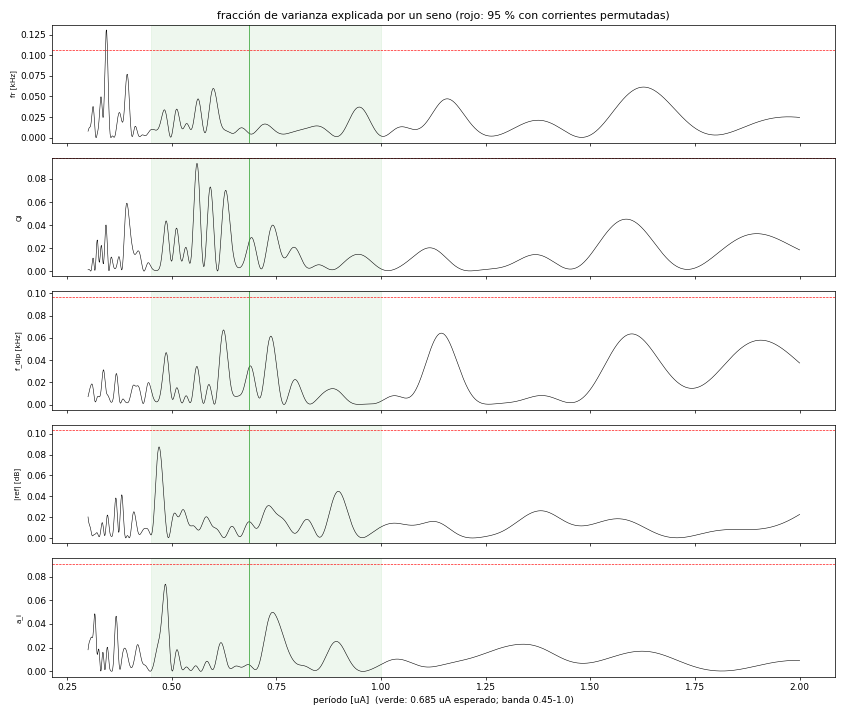
\includegraphics[width=0.75\textwidth]{periodo_resonador.png}
\caption{Fracción de varianza explicada por un seno en función del período, para los parámetros del resonador
(runs 50--177). La línea roja es el umbral de 95\,\% con corrientes permutadas; la banda verde marca 0.45--1.0\,$\mu$A.}
\label{fig:per}
\end{figure}

\subsection{Un tono en CW con paso fino (runs 233--238)}

Se fijó $f_{\rm CW}$ sobre el flanco del resonador y se barrió la corriente de 0 a $-2\uA$ en pasos de $5\,$nA
($\approx 0.007\,\Phi_0$ si $P = 0.69\uA$), con el VNA a $-20\dBm$ e IFBW de 1\,Hz. Cada punto se convirtió en
$\dfr$ y se analizó con FFT, periodograma de seno con nulo de ruido rojo AR(1), pruebas a período fijo y comparación
entre runs repetidos.

\begin{table}[H]
\centering
\small
\begin{tabularx}{\textwidth}{c c c X}
\toprule
Run & Resonador & Puntos CW & Resultado \\
\midrule
233 & res\_q1 & 1  & pico marginal en $P = 0.514\uA$ (p global $\approx 0.08$); no se repitió \\
234 & res\_q4 & 1  & nada \\
235 & res\_q4 & 5  & $4.9\pm1.2\kHz$ en $P = 0.549\uA$; \textbf{no se reprodujo en el 236} \\
236 & res\_q4 & 10 & deriva lenta de $\pm20\kHz$; en $0.549\uA$ da $0.2$--$3.4\kHz$ según la línea de base \\
237 & res\_q2 & 1  & ruido $\sim 42\kHz$ por punto; bulto de 1.2--1.6\,$\mu$A del tamaño del barrido (deriva) \\
238 & res\_q2 & 3  & ruido $\sim 22\kHz$; nada; curvas lentas \textbf{anticorrelacionadas} con el 237 ($-0.76$) \\
\bottomrule
\end{tabularx}
\caption{Espectroscopía de un tono con paso fino.}
\end{table}

\textbf{Cotas:} cualquier modulación de $\fr$ con el flujo es menor que $\sim 3$--$4\kHz$ en res\_q4 (períodos de 0.4 a
$0.8\uA$) y que $\sim 4$--$5\kHz$ en res\_q2 (0.5 a $1.6\uA$).

\textbf{Deriva:} $\fr$ deriva decenas de kHz en decenas de minutos y cientos de kHz en horas. En un barrido lento esa
deriva imita períodos de $\sim 1\uA$; por eso los indicios aislados (233, 235) no se reprodujeron. Es mejor repetir
barridos rápidos iguales y promediarlos, porque la deriva cambia de una repetición a otra (figura~\ref{fig:repro}).

\begin{figure}[H]
\centering
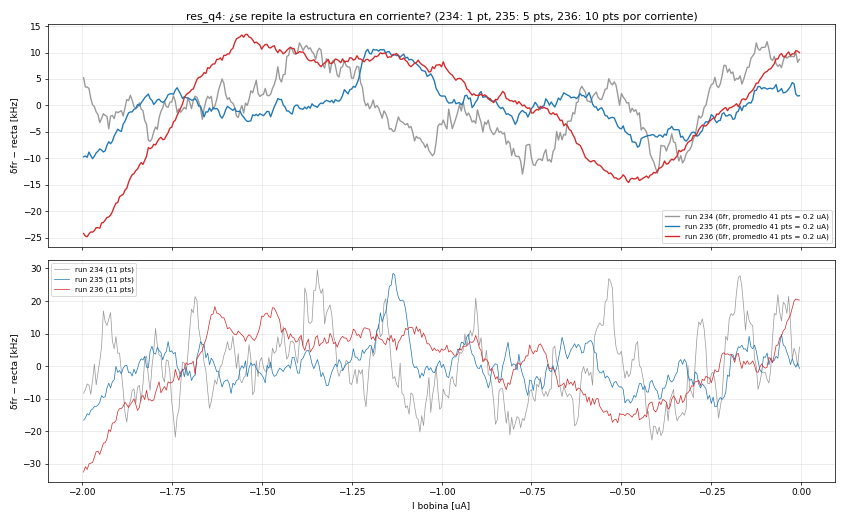
\includegraphics[width=0.49\textwidth]{reproduce_q4.png}\hfill
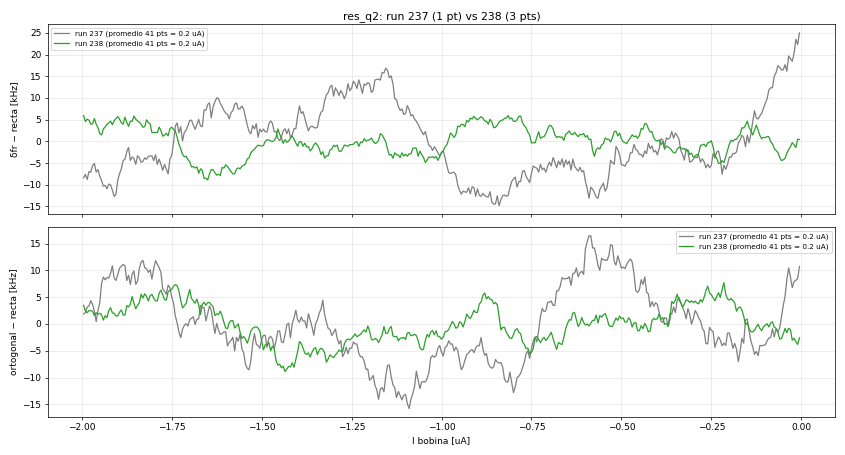
\includegraphics[width=0.49\textwidth]{reproduce_q2.png}
\caption{Reproducibilidad de los runs de un tono: res\_q4 (234--236, izquierda) y res\_q2 (237 contra 238,
derecha). Las estructuras lentas no se repiten entre runs.}
\label{fig:repro}
\end{figure}

%==============================================================================
\section{Espectroscopía de dos tonos}
%==============================================================================

En todas las mediciones de dos tonos, en cada corriente: (1) con el drive apagado se ubica el mínimo del resonador y
se fija $f_{\rm CW}$; (2) se toma una referencia sin drive; (3) se barre la frecuencia del drive leyendo $S_{21}$ en CW.
Cada corriente es un run de QCoDeS.

\subsection{Barridos gruesos (runs 1--230)}

Drive de 0.1 a $13\GHz$, entre $-20$ y $+10\dBm$ a la salida del generador, en corrientes alrededor de 0, $-21$,
$-125$ y $-139\uA$, con pasos de 0.1 a $1\uA$.

\begin{itemize}
  \item Con drive de $+10\dBm$ aparecen caídas de $|S_{21}|$ sin cambio de fase cerca de 5.0, 5.41, 6.07 y
    $6.4\GHz$ (figura~\ref{fig:hemt}). No dependen de la corriente. Se interpretan como compresión del HEMT: el drive
    que se acopla a la línea de salida llega al amplificador, lo satura y le baja la ganancia.
  \item No aparece ninguna línea que siga al flujo. Una línea con $|\Delta S_{21}| \gtrsim 0.13$ ($\sim 1\dB$) se
    habría visto en los mapas de 4--8\,GHz.
  \item Con pasos de 0.1--1\,$\mu$A (0.15--1.5\,$\Phi_0$ si $P \approx 0.69\uA$) el flujo quedaba muestreado de forma
    muy gruesa; esto motivó los barridos finos.
\end{itemize}

\begin{figure}[H]
\centering
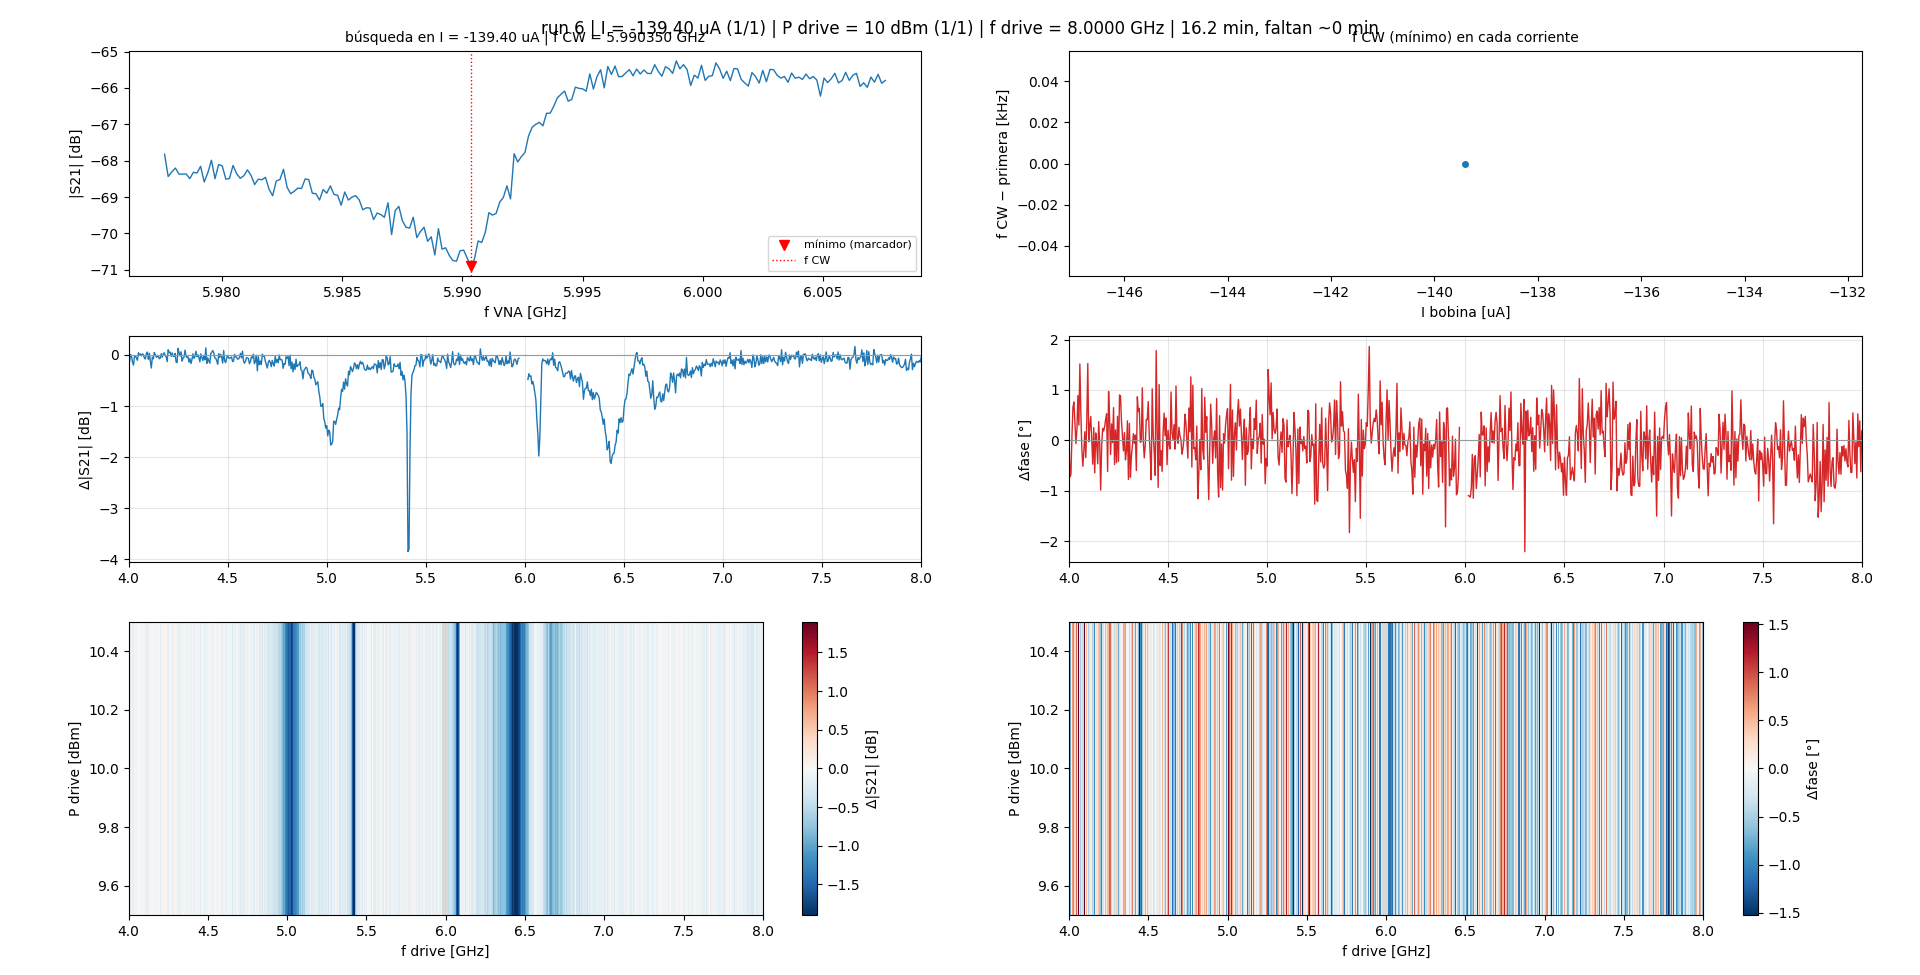
\includegraphics[width=0.85\textwidth]{vivo_run6_4-8GHz.png}
\caption{Run 6: drive de 4 a $8\GHz$ a $+10\dBm$. Las caídas de $\Delta|S_{21}|$ sin cambio de fase son compresión
del amplificador, no transiciones del qubit.}
\label{fig:hemt}
\end{figure}

\subsection{Barrido fino a 0\,dBm (runs 239--619)}

Drive de $1\MHz$ a $4\GHz$ (paso de $5\MHz$) a $0\dBm$, VNA a $-20\dBm$, 1 punto CW a 10\,Hz, $f_{\rm CW}$ fija
($2.1\MHz$ debajo de $\fr$), y 381 corrientes de $-0.005$ a $-1.905\uA$ en pasos de 5\,nA (14.5\,h).

\begin{itemize}
  \item Ruido: $116\kHz$ por punto en $\dfr$. Agrupando de a 10 corrientes (50\,nA) baja a $36\kHz$, como ruido
    blanco.
  \item Después de restar el fondo común, ninguna de las $\sim 30\,000$ celdas pasa $4.5\sigma$
    (figura~\ref{fig:mapa}). El fondo común no tiene líneas fijas por encima de $\sim 25\kHz$.
  \item Dos curvas marcadas a ojo sobre el mapa en vivo (una recta de $0.62$ a $0.10\GHz$ y dos curvas en V con
    mínimo en $-0.31\uA$) se analizaron con búsqueda de rectas con nulo, validación cruzada entre corrientes pares e
    impares, autocorrelación 2D e inyección de líneas sintéticas. Ninguna resultó significativa: el ojo encuentra
    estructuras en el ruido; una línea real de $0.08\dB$ casi no se distingue a simple vista pero el método la
    detecta con $z \approx 6$.
  \item En el promedio de $\fr$ (referencia sin drive) hay una deriva de $-350$ a $+390\kHz$ en 14.5\,h, sin período
    estable.
\end{itemize}

\begin{figure}[H]
\centering
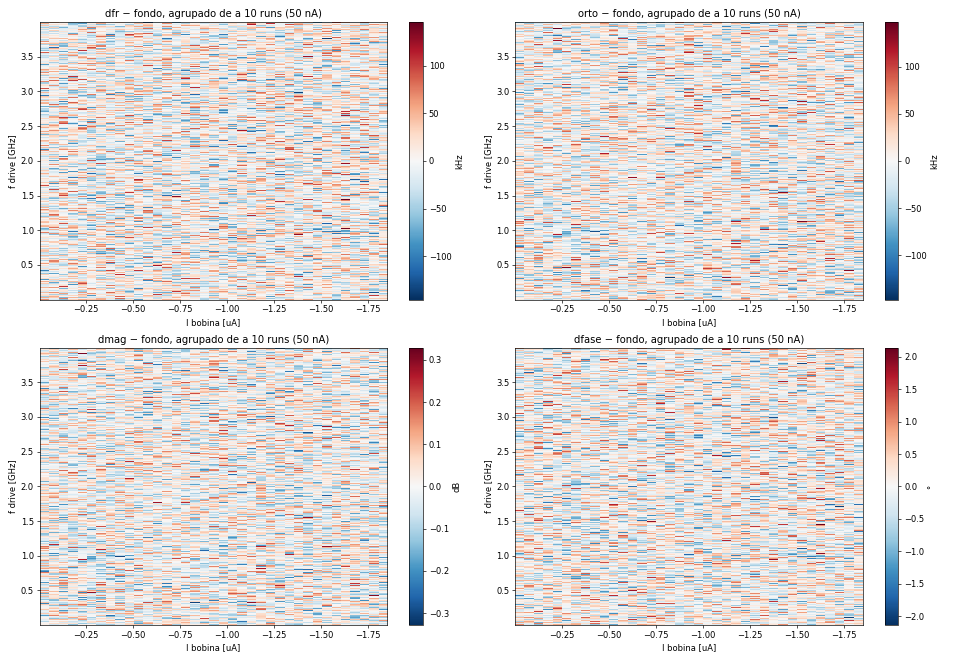
\includegraphics[width=0.8\textwidth]{mapa_todo.png}
\caption{Runs 239--619: mapas de $\dfr$, componente ortogonal, $\Delta|S_{21}|$ y $\Delta$fase con el fondo común
restado, agrupados de a 10 corrientes. Solo ruido.}
\label{fig:mapa}
\end{figure}

\subsection{Barrido sensible (runs 681--713)}

Se cambió la estrategia para maximizar la sensibilidad:
\begin{itemize}
  \item VNA a $0\dBm$ ($\langle n\rangle \approx 17$, inofensivo para un qubit muy desacoplado) y 10 puntos CW a 10\,Hz;
  \item $f_{\rm CW}$ en $\fr$, donde la pendiente de $S_{21}$ es máxima;
  \item drive a $+10\dBm$, de 1\,MHz a 4\,GHz en pasos de 5\,MHz;
  \item una sola búsqueda del mínimo al principio y $f_{\rm CW}$ fija (ahorra tiempo);
  \item 33 corrientes de $-0.005$ a $-0.805\uA$ en pasos de 25\,nA: más de un período si $P$ está entre 0.5 y
    $0.7\uA$ (8.5\,h, solo ida).
\end{itemize}

El ruido bajó a $\sim 2\kHz$ por punto en $\dfr$, unas 60 veces menos que el barrido anterior, y a $0.35\kHz$
promediando las 33 corrientes.

\begin{figure}[H]
\centering
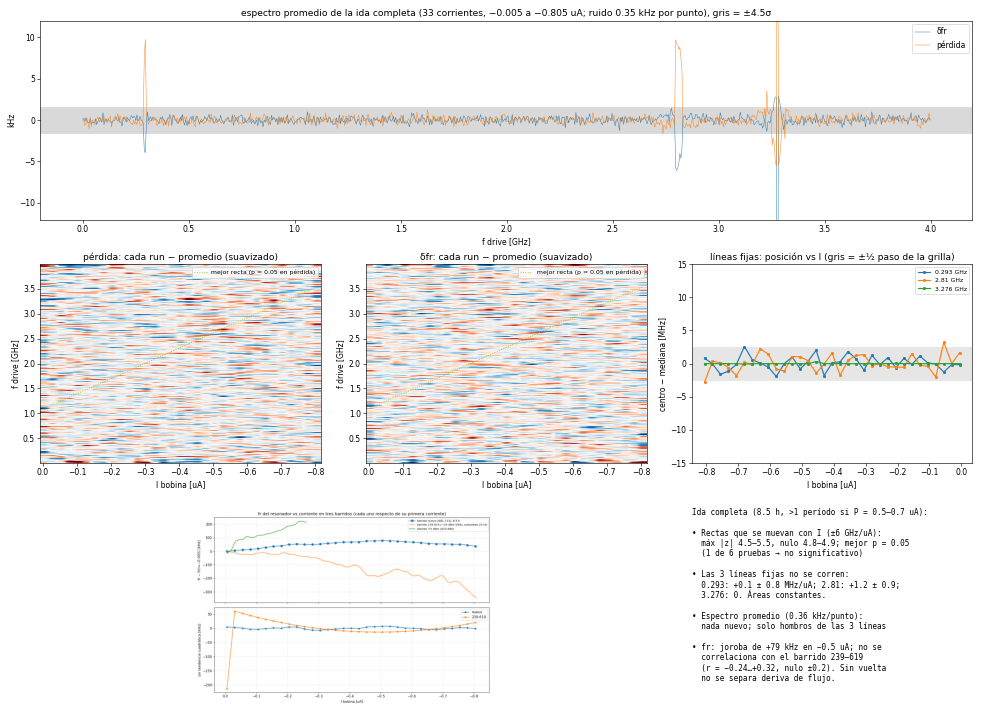
\includegraphics[width=0.95\textwidth]{ida_681-713.png}
\caption{Runs 681--713. Arriba: espectro promedio (gris: $\pm4.5\sigma$). Medio: lo que cambia entre corrientes
($\dfr$ y pérdida, cada run menos el promedio) y la posición de las líneas fijas en función de la corriente.
Abajo: $\fr$ del resonador comparado con barridos anteriores.}
\label{fig:ida}
\end{figure}

\paragraph{Tres líneas fijas.} Aparecen en todas las corrientes (figuras~\ref{fig:ida} y~\ref{fig:lineas}):

\begin{table}[H]
\centering
\begin{tabular}{l l c c c}
\toprule
Línea & Forma & $\dfr$ & Pérdida & Variación con $I$ \\
\midrule
$0.293\GHz$ & 2 puntos de la grilla ($\le 10\MHz$) & $-4\kHz$ & $+9\kHz$ & $+0.1\pm0.8\MHz/\mu\mathrm{A}$ \\
$2.81\GHz$ & rectangular, 2.796--2.826\,GHz & $-5\kHz$ & $+9\kHz$ & $+1.2\pm0.9\MHz/\mu\mathrm{A}$ \\
$3.276\GHz$ & 1 punto, hombros de $\pm50\MHz$ & $-40\kHz$ & $+46\kHz$ & ninguna \\
\bottomrule
\end{tabular}
\caption{Líneas fijas del barrido sensible. Las tres tienen el resonador hacia abajo y más pérdida.}
\end{table}

\begin{figure}[H]
\centering
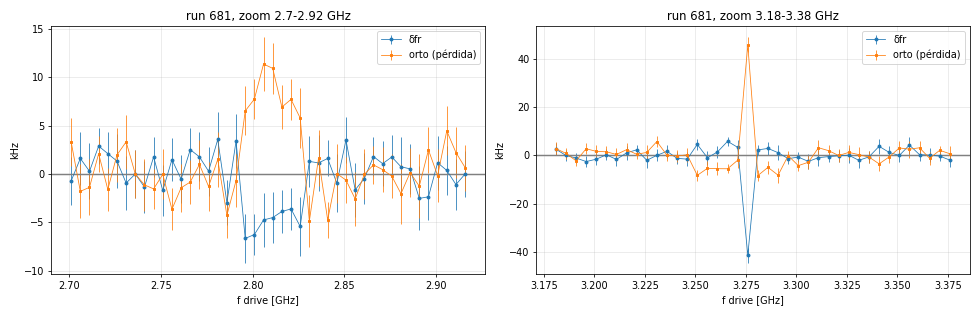
\includegraphics[width=0.85\textwidth]{lineas_fijas_run681.png}
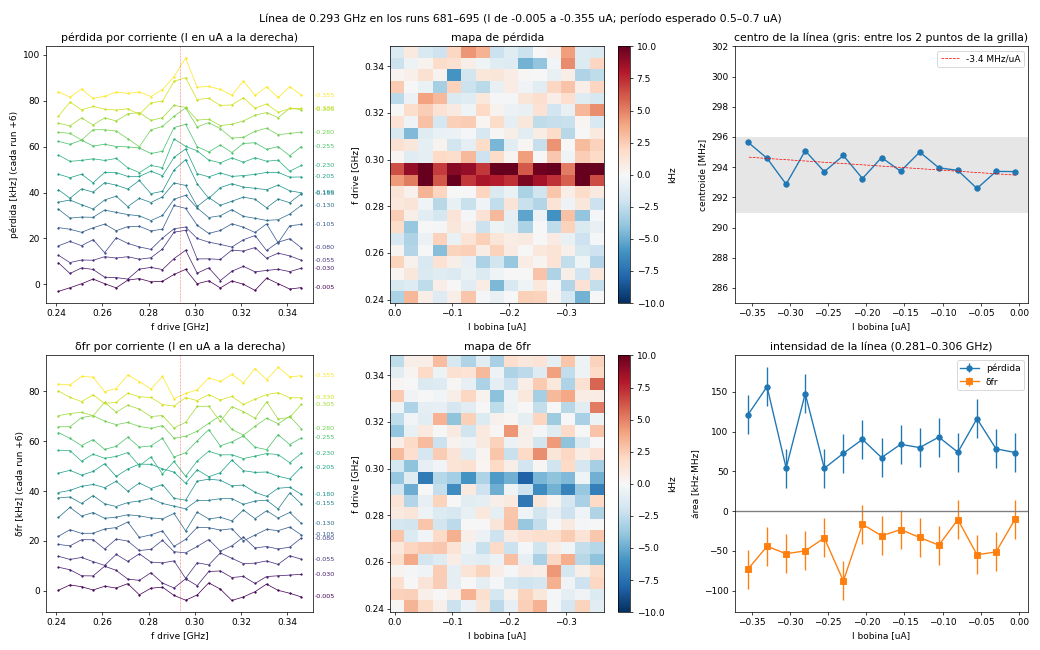
\includegraphics[width=0.95\textwidth]{linea_0293.png}
\caption{Arriba: zoom de las líneas de 2.81 y $3.276\GHz$ en el run 681. Abajo: la línea de $0.293\GHz$ en las
primeras 15 corrientes: espectros, mapas, centroide e intensidad en función de la corriente.}
\label{fig:lineas}
\end{figure}

La línea de $0.293\GHz$ tiene la frecuencia que se esperaría para la $f_{01}$ de un fluxonium cerca de medio flujo,
pero no se mueve: en $0.8\uA$, más de un período esperado, su centro cambia menos de $\sim 1\MHz$ (si se corriera
aunque sea 1\,MHz, uno de sus dos puntos ganaría intensidad y el otro perdería, y eso no pasa). Un fluxonium se
correría cientos de MHz en ese rango. La de $3.276\GHz$ ya se había visto fija en los barridos gruesos a
corrientes de decenas de $\mu$A.

\paragraph{Búsqueda sin supuestos.} Como el chip no salió como se esperaba, se buscó cualquier dependencia con la
corriente sin suponer período ni forma (figura~\ref{fig:busqueda}), siempre con un nulo construido con los mismos
datos desordenados:
\begin{itemize}
  \item posición fina, ancho y forma de las líneas fijas (cociente entre puntos vecinos, bordes, componentes
    principales);
  \item cada frecuencia de drive (y ventanas de 15 y 45\,MHz): tendencia, curvatura y seno de período 0.05--1.6\,$\mu$A;
  \item rectas de hasta $\pm6\GHz/\mu\mathrm{A}$;
  \item trayectorias libres por programación dinámica, con saltos de 5 a 400\,MHz entre corrientes.
\end{itemize}
Nada supera lo esperable por azar. La mejor trayectoria libre no se reproduce entre corrientes pares e impares.

\begin{figure}[H]
\centering
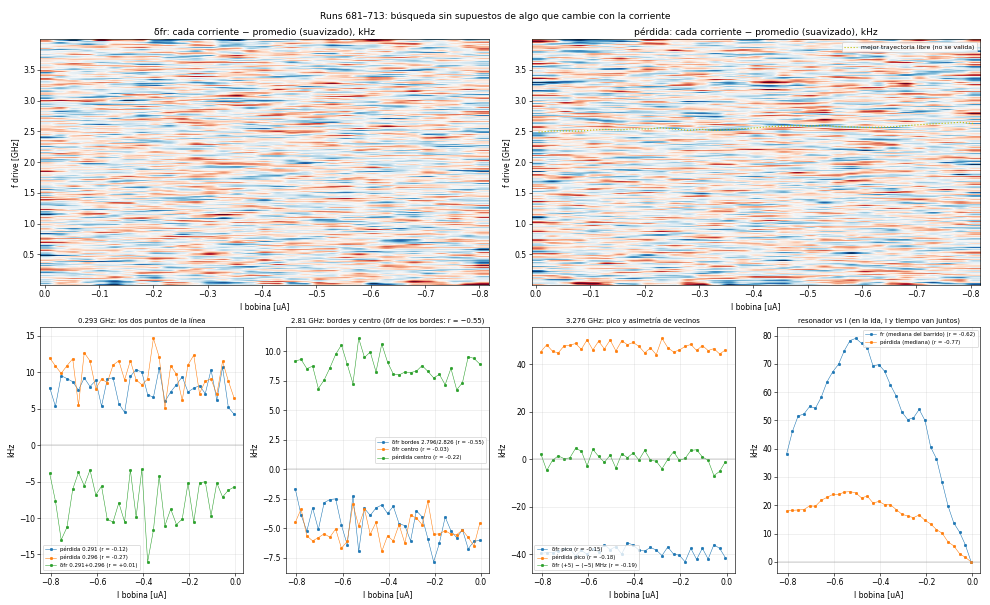
\includegraphics[width=0.95\textwidth]{busqueda_sin_supuestos_681-713.png}
\caption{Búsqueda sin supuestos en los runs 681--713: lo que cambia entre corrientes, la mejor trayectoria libre
(que no se valida), las líneas fijas y el resonador en función de la corriente.}
\label{fig:busqueda}
\end{figure}

\subsection{Prueba de control: corriente contra tiempo (runs 714--723)}

En la ida la corriente y el tiempo avanzan juntos, así que una tendencia con la corriente puede ser deriva. Quedaban
dos indicios débiles: los bordes de la línea de 2.81\,GHz en $\dfr$ ($r = -0.55$ con $I$) y una curvatura en
$2.996\GHz = f_{\rm CW}/2$ (el segundo armónico del drive cae sobre el resonador). Se midieron de nuevo 5 corrientes
dos veces cada una en orden alternado (correlación entre corriente y tiempo de 0.10), con 30 puntos CW
(figura~\ref{fig:prueba}):
\begin{itemize}
  \item bordes de 2.81\,GHz: $+0.8\pm1.7\kHz/\mu\mathrm{A}$, contra $-3.7\kHz/\mu\mathrm{A}$ en la ida; en cambio
    se corren con el tiempo ($-1.75\pm0.68\kHz$ entre pasadas a la misma corriente). Era deriva;
  \item $2.996\GHz$: la forma de la ida aparece con amplitud $-0.2\pm0.6$ (1 sería igual). No se repite.
\end{itemize}

\begin{figure}[H]
\centering
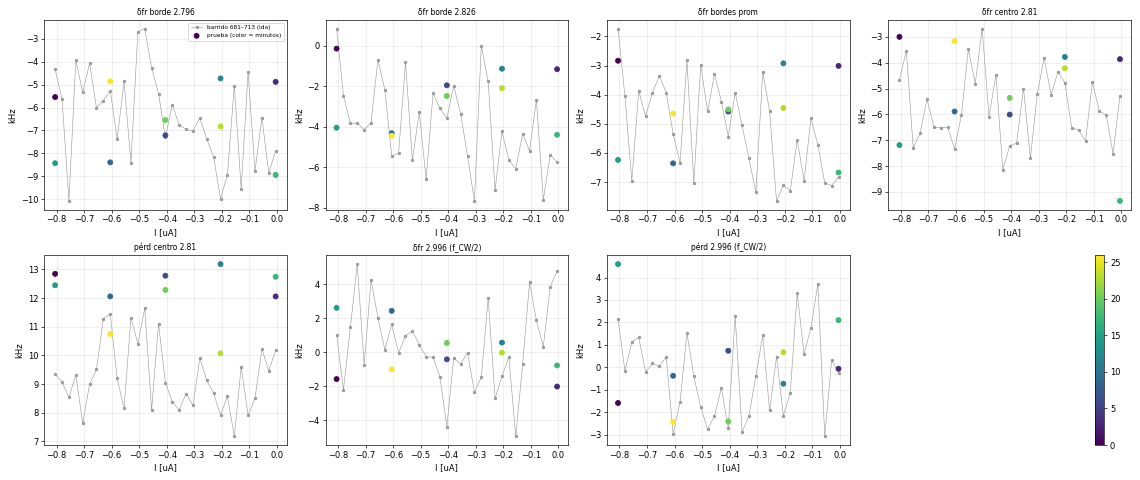
\includegraphics[width=0.95\textwidth]{prueba_I_vs_tiempo_714-723.png}
\caption{Prueba de control (puntos de colores; el color indica los minutos desde el inicio) sobre los valores del
barrido sensible (gris). Ninguno de los indicios sigue a la corriente.}
\label{fig:prueba}
\end{figure}

%==============================================================================
\section{Temperatura de la placa de mezcla}
\label{sec:temperatura}
%==============================================================================

Los logs del Bluefors muestran que la placa de mezcla se calienta con la potencia de las mediciones
(figura~\ref{fig:temp}): $8.05\mK$ con drive de $0\dBm$ y VNA a $-20\dBm$; $\approx 8.5\mK$ con drive de
$+5\dBm$; $\approx 9.3\mK$ con drive de $+10\dBm$ y VNA a $0\dBm$; y $\approx 10\mK$ durante los barridos gruesos
con drive hasta 10\,GHz. Al frenar la medición vuelve a $8.0\mK$ en $\sim 1.5$\,h. El still se mantiene en
$\approx 835\mK$. Este calentamiento no afecta las conclusiones, pero muestra que el drive deposita potencia en el
chip o su entorno.

\begin{figure}[H]
\centering
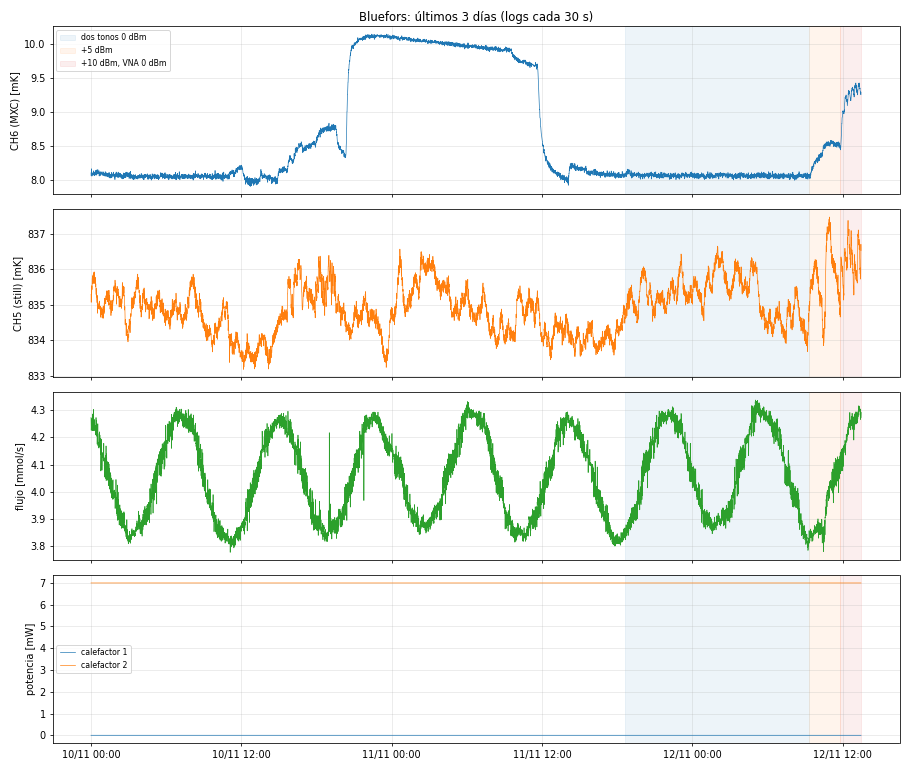
\includegraphics[width=0.85\textwidth]{temperaturas.png}
\caption{Temperaturas de la placa de mezcla (CH6) y del still (CH5), flujo y calefactores durante los últimos
barridos de dos tonos (franjas de colores).}
\label{fig:temp}
\end{figure}

%==============================================================================
\section{Hipótesis físicas sobre lo medido}
\label{sec:hipotesis}
%==============================================================================

\subsection{Ramas con histéresis: un lazo superconductor con estados de fluxoide metaestables}

Las ramas parabólicas desplazadas un período, con saltos y ventanas de existencia que se solapan, son la firma de un
lazo superconductor que atrapa un número entero de cuantos de flujo (fluxoides) y salta de estado cuando la corriente
que circula supera un valor crítico. Dentro de cada estado la corriente circulante es proporcional a $(I - C_n)$, y
el resonador se corre como su cuadrado (por inductancia cinética o por la no linealidad de un tramo compartido), lo
que da las parábolas. Que existan 2--3 estados a la vez y que el patrón dure horas implica un lazo fuertemente
histerético (tipo rf-SQUID con $\beta_L \gg 1$) en el que casi no hay saltos de fase espontáneos.

Hay dos lecturas posibles, según qué lazo sea:
\begin{enumerate}
  \item \textbf{No es el lazo del qubit.} Con la calibración de la bobina ($P_{\rm esp} \approx 0.69\uA$ para
    $2700\,\mu\mathrm{m}^2$), un período de $50\uA$ corresponde a un lazo de $\sim 37\,\mu\mathrm{m}^2$, que tendría
    que ser alguna otra estructura (por ejemplo, un lazo formado por el resonador o la línea de flujo con el plano de
    tierra). Como aparece con el mismo período en res\_q2 y res\_q4, sería una estructura repetida en el diseño.
  \item \textbf{Es el lazo del qubit, y el acople de la bobina a este chip es mucho menor que en la muestra de
    calibración} (factor $\sim 70$). Entonces el fluxonium se comporta como un rf-SQUID clásico: con
    $E_J/E_L \approx 10$ hay varios mínimos de energía potencial, y si la juntura chica quedó más grande de lo
    diseñado ($E_J/E_C$ alto), el tunneling entre pozos (los saltos de fase cuánticos que hacen al fluxonium un qubit)
    queda suprimido. El circuito queda atrapado en un pozo, salta de forma clásica y su transición $0\to1$ dentro de
    un pozo es la del plasma, a frecuencias altas y con elementos de matriz muy chicos hacia la lectura. En este caso
    no hay qubit fluxonium funcionando aunque el lazo esté cerrado.
\end{enumerate}

\subsection{Oscilación de $23.8\uA$}

Es suave y sin histéresis, solo existe en res\_q4 y desaparece con muchos fotones. Es compatible con un elemento
no lineal (por ejemplo un lazo con una juntura en régimen no histerético, o defectos que se saturan) acoplado
débilmente solo al resonador de Q4. Que no aparezca en res\_q2, que tiene el mismo diseño de qubit, indica algo local
de esa zona del chip (un defecto de fabricación, un vórtice atrapado cerca, o un lazo parásito), no del diseño. Con la
calibración de la bobina su período corresponde a $\sim 80\,\mu\mathrm{m}^2$, tampoco el área del fluxonium.

\subsection{Líneas fijas en dos tonos}

Las líneas de 0.293, 2.81 y $3.276\GHz$ bajan $\fr$ y aumentan la pérdida, que es lo que produce un calentamiento
local (cuasipartículas o TLS excitados) o la absorción de potencia de drive. Además la placa de mezcla se calienta
con el drive. Lo más probable es que sean frecuencias en las que el drive se acopla mejor al chip: modos de la caja o
de la antena, ondas estacionarias en la línea de drive, o defectos (TLS). La de $2.81\GHz$, rectangular y de bordes
abruptos, se parece más a un artefacto del generador (un espurio o un cambio de banda interna). Ninguna depende del
flujo, así que no son transiciones de un fluxonium sintonizable.

\subsection{Caídas de $|S_{21}|$ con drive alto entre 5 y 6.5\,GHz}

Solo en magnitud, sin fase, y sin dependencia con la corriente: compresión de ganancia del HEMT por el drive que
llega a la cadena de salida.

\subsection{Deriva lenta de $\fr$}

Decenas de kHz por hora, con ondulaciones. Es típica de resonadores con pérdidas dieléctricas (fluctuación de TLS) o
cambios lentos de cuasipartículas y temperatura; impone repetir mediciones para separar flujo de tiempo.

%==============================================================================
\section{Por qué no se puede confirmar que haya un qubit funcionando}
%==============================================================================

\begin{enumerate}
  \item \textbf{No hay ninguna señal que dependa del flujo con la periodicidad de un qubit.} En un tono la modulación
    de $\fr$ es menor que $\sim 3$--$5\kHz$ en el rango de períodos esperado. En dos tonos, entre 1\,MHz y 4\,GHz y
    a lo largo de más de un período esperado, nada se corre más de $\sim 3$--$4\kHz$ con la corriente.
  \item \textbf{Las únicas líneas espectrales están fijas.} Una transición de fluxonium se movería cientos de MHz en
    ese rango de flujo; las líneas encontradas se mueven menos de $\sim 1\MHz$ y tienen la firma de absorción o de
    artefactos.
  \item \textbf{Las estructuras que sí dependen del flujo no tienen la forma de un qubit.} Las ramas son
    histeréticas y clásicas, y la oscilación de $23.8\uA$ es local y desaparece con la potencia; ninguna de las dos
    tiene un período compatible con la calibración de la bobina para el lazo del fluxonium.
  \item \textbf{La señal puede estar por debajo de la sensibilidad.} Con los qubits muy desacoplados, $\chi$ podría
    ser menor que los $\sim 3\kHz$ alcanzados, y a baja frecuencia el contraste térmico reduce todavía más la señal.
  \item \textbf{Hay rangos no cubiertos.} La transición podría estar por encima de $4\GHz$ en el barrido sensible
    (los barridos de 4--13\,GHz fueron mucho menos sensibles), o ser más angosta que el paso de 5\,MHz cerca de un
    punto dulce. El período real podría ser distinto del estimado si la bobina no acopla como en la muestra de
    calibración.
  \item \textbf{Los defectos de fabricación pueden haber dejado al qubit fuera de régimen:} juntura chica con
    $E_J/E_C$ demasiado alto (sin tunneling, comportamiento de rf-SQUID), arreglo de junturas dañado, o lazo abierto.
    Ninguna medición permite distinguir estos casos de un qubit funcionando pero indetectable.
\end{enumerate}

%==============================================================================
\section{Resumen de lo realizado y obtenido}
%==============================================================================

\begin{table}[H]
\centering
\small
\begin{tabularx}{\textwidth}{l l X}
\toprule
Medición & Runs / base & Resultado \\
\midrule
Resonadores $\lambda/4$ y $\lambda/2$ & \texttt{fluxonium\_database}, \texttt{resonadores\_vna.db} & $\fr$, $Q$ y $\kappa$ de res\_q1, q2, q4; $Q$ bajos \\
Barridos de corriente & \texttt{punch\_out.db} & ramas de fluxoide histeréticas ($T\approx50\uA$), independientes de la potencia; oscilación de $23.8\uA$ solo en res\_q4 \\
Dos tonos gruesos & \texttt{two\_tone\_flux2.db}, 1--230 & compresión del HEMT; sin líneas que dependan del flujo \\
Un tono fino & 233--238 & modulación de $\fr$ $<3$--$5\kHz$; indicios aislados no reproducibles (deriva) \\
Dos tonos fino & 239--619 & ruido $116\kHz$; nada por encima de $\sim 80$--$150\kHz$ \\
Dos tonos sensible & \texttt{two\_tone\_flux2\_651-723.db}, 681--713 & ruido $2\kHz$; tres líneas fijas; nada dependiente del flujo $>3$--$4\kHz$ \\
Control corriente/tiempo & 714--723 & los indicios restantes eran deriva \\
\bottomrule
\end{tabularx}
\caption{Resumen de las mediciones.}
\end{table}

\paragraph{Lo que se aprendió sobre cómo medir.}
\begin{itemize}
  \item Con qubits muy desacoplados conviene leer con más fotones (el número crítico es alto) y en $\fr$, mirando la
    fase o $\dfr$ y no $|S_{21}|$, que en el mínimo es casi insensible a un corrimiento.
  \item Pocas corrientes con mucho promedio rinden más que muchas corrientes con un punto: el análisis con plantillas
    a lo largo de las corrientes recupera la sensibilidad.
  \item La deriva lenta de $\fr$ obliga a medir en orden alternado o con ida y vuelta para separar flujo de tiempo.
  \item Los patrones que se ven a ojo en mapas ruidosos deben validarse con nulos y con datos independientes.
\end{itemize}

\paragraph{Pasos posibles para resolver si hay un qubit.}
\begin{itemize}
  \item Medir con la configuración sensible el rango de 4 a 13\,GHz (o hasta donde llegue el generador).
  \item Confirmar la constante de la bobina en este chip (por ejemplo, con una estructura de área conocida) para
    saber qué período corresponde al fluxonium.
  \item Caracterizar en DC o a temperatura ambiente las junturas de una muestra hermana, para ver si $E_J$ y $E_C$
    quedaron dentro del régimen fluxonium.
  \item Repetir el barrido sensible con ida y vuelta, y en un rango de corriente más amplio.
\end{itemize}

\paragraph{Conclusión.} El chip muestra un lazo superconductor con estados de fluxoide metaestables y, en Q4, un
elemento no lineal adicional, pero ninguna medición mostró una transición de qubit que dependa del flujo. Con la
sensibilidad alcanzada ($\sim 3$--$4\kHz$ en dos tonos hasta $4\GHz$) no se puede confirmar que haya un qubit
fluxonium funcionando.

\appendix
\section{Datos y código}

Todo está en el repositorio \texttt{ezequiel1611/fluxonium}:
\begin{itemize}
  \item \texttt{codigo/}: \texttt{vna\_single.py}, \texttt{barrido\_flujo.py}, \texttt{fit\_resonancia.py},
    \texttt{fotones\_resonador.py} y \texttt{dos\_tonos.py} (\texttt{medir\_dos\_tonos}, \texttt{medir\_un\_tono} y
    sus cargadores).
  \item \texttt{notebooks/}: \texttt{readout.ipynb}, \texttt{medir\_resonadores.ipynb}, \texttt{punch\_out.ipynb} y
    \texttt{two\_tone\_flux2.ipynb}.
  \item \texttt{datos/}: bases QCoDeS por Git LFS. Los runs de dos tonos y un tono están en
    \texttt{two\_tone\_flux2/two\_tone\_flux2.db} (runs 1--650) y \texttt{two\_tone\_flux2\_651-723.db} (runs 651--723),
    sin los runs cortados.
  \item \texttt{informes/}: los informes de los barridos de corriente de res\_q4, el resumen de la búsqueda del qubit
    (\texttt{dos\_tonos/README.md}) y este informe.
\end{itemize}

\end{document}
